%% LyX 2.3.5.2 created this file.  For more info, see http://www.lyx.org/.
%% Do not edit unless you really know what you are doing.
\documentclass[english]{extarticle}
\usepackage[T1]{fontenc}
\usepackage[latin9]{inputenc}
\usepackage{calc}
\usepackage{url}
\usepackage{amsmath}
\usepackage{amsthm}
\usepackage{graphicx}

\makeatletter
%%%%%%%%%%%%%%%%%%%%%%%%%%%%%% Textclass specific LaTeX commands.
\numberwithin{equation}{section}
\numberwithin{figure}{section}
\theoremstyle{plain}
\newtheorem{thm}{\protect\theoremname}
\theoremstyle{definition}
\newtheorem{defn}[thm]{\protect\definitionname}
\theoremstyle{plain}
\newtheorem{fact}[thm]{\protect\factname}
\theoremstyle{plain}
\newtheorem{lem}[thm]{\protect\lemmaname}

\makeatother

\usepackage{babel}
\providecommand{\definitionname}{Definition}
\providecommand{\factname}{Fact}
\providecommand{\lemmaname}{Lemma}
\providecommand{\theoremname}{Theorem}

\begin{document}
\title{The simplest unsolved computational geometry problem: efficiently
folding a polyhedron}
\author{Linus Hamilton\thanks{Supported by a Fannie and John Hertz Fellowship.}
\and Yevhenii Diomidov}
\maketitle
\begin{abstract}
What is the smallest square of paper that can wrap around the surface
of a given polyhedron? We develop a method to find upper bounds for
this problem, and use it to find new record foldings for the tetrahedron,
octahedron, dodecahedron, and icosahedron. We present evidence that
the tetrahedron folding is optimal.

We released the code of our algorithm: \url{https://github.com/6849-2020/efficient-polyhedra-folds/blob/main/foldingPolyhedra.py}.
\end{abstract}

\section{Introduction}

Many computational geometry problems present themselves so simply
that they ought to be solved by now. For example, Moser's worm problem
\cite{norwood1992worm} (what is the smallest shape that contains
any length-1 curve?), or the moving sofa problem \cite{wagner1976sofa}
(what is the smallest shape that fits through a $90^{\circ}$ turn
in a hallway?). It speaks to a fundamental gap in the field of computational
geometry that we have not been able to answer these questions.

In this paper we study a similarly simple question: what is the smallest
square of paper that wraps completely around the surface of a given
polyhedron? We pay special attention to the simplest case, that of
the tetrahedron, for which this may be a contender for the ``easiest
unsolved computational geometry problem.'' Unlike the sofa and worm
conundrums, folding a square around a tetrahedron seems, at least
intuitively, to have finitely many degrees of freedom. Yet, even though
we present evidence that our new tetrahedron fold is optimal, the
answer is still not known for sure.

In this paper, we present a method to search for efficient foldings
of arbitrary polyhedra. We demonstrate the power of our method by
improving the best known records for wrapping a square around a tetrahedron,
octahedron, dodecahedron, and icosahedron. (The answer for a cube
was already known to be optimal.) This is similar to the research
in \cite{cole2013wrapping}, which studies wrapping a cube or a sphere
using the smallest possible rectangle with a given length/width ratio.
We also explore a technique, novel to this author, to obtain a restricted
lower bound on tetrahedron wrapping. The technique may be useful on
other computational geometry problems.

\section{The tetrahedron}

For the purpose of exposition, we will first demonstrate our method
on the tetrahedron.

Consider this 4-colored tiling of unit equilateral triangles:
\begin{center}
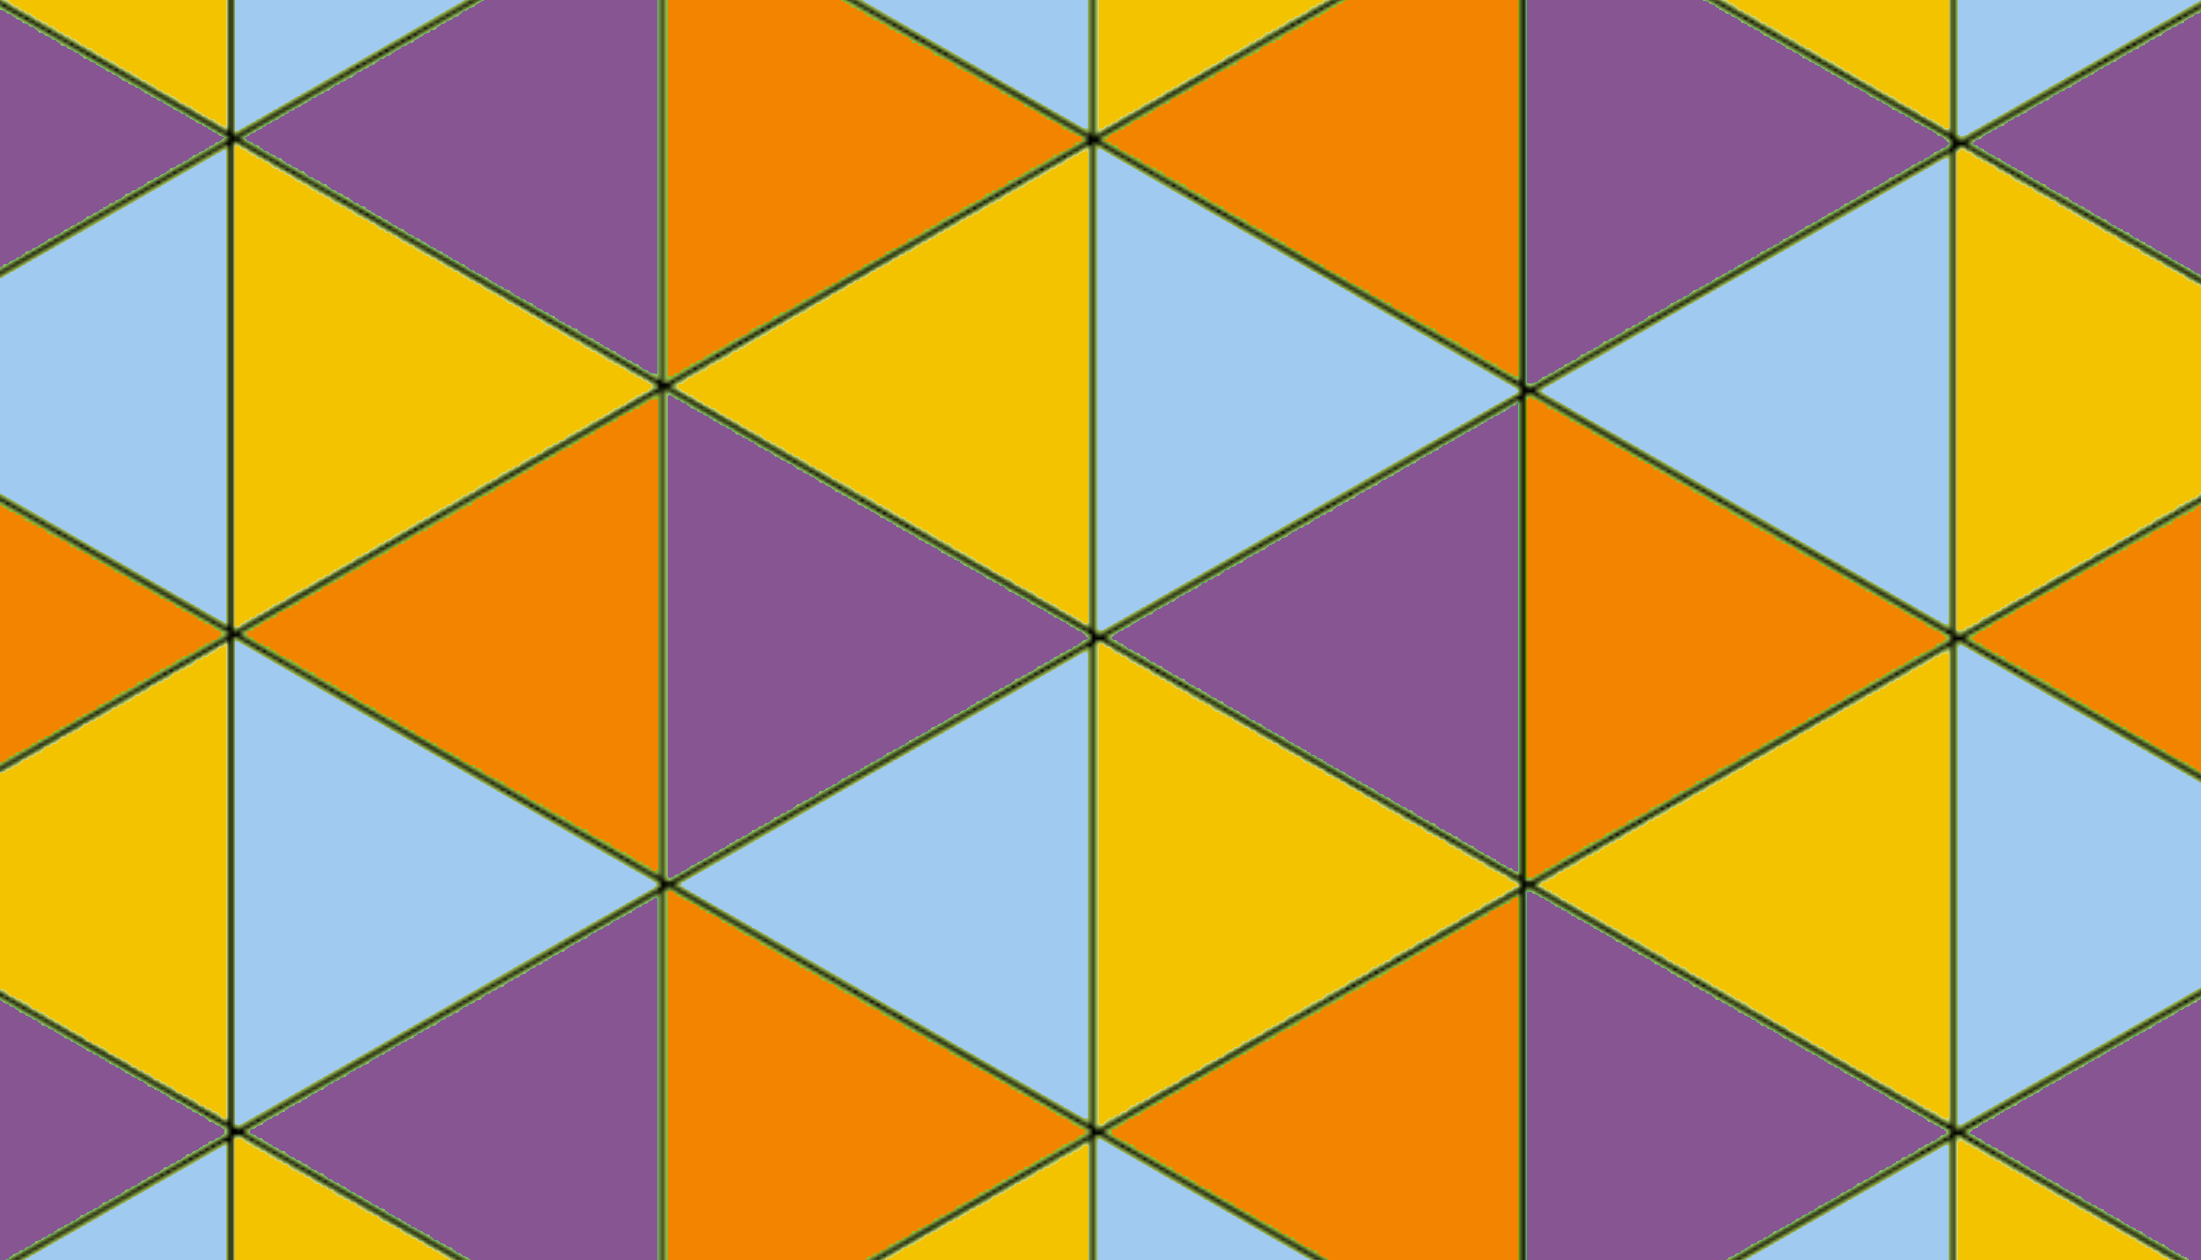
\includegraphics[scale=0.5]{triangle_land}
\par\end{center}

Surprisingly, if the paper is allowed to intersect itself, this tiling
folds perfectly onto the surface of a unit tetrahedron, with each
color corresponding to one face. This is because every vertex of a
tetrahedron has total face degree $\pi=\tau/2$, so every vertex of
the above tiling double-covers a tetrahedron vertex.

Now examine the following square. Two pairs of equal-length segments
are marked.
\begin{center}
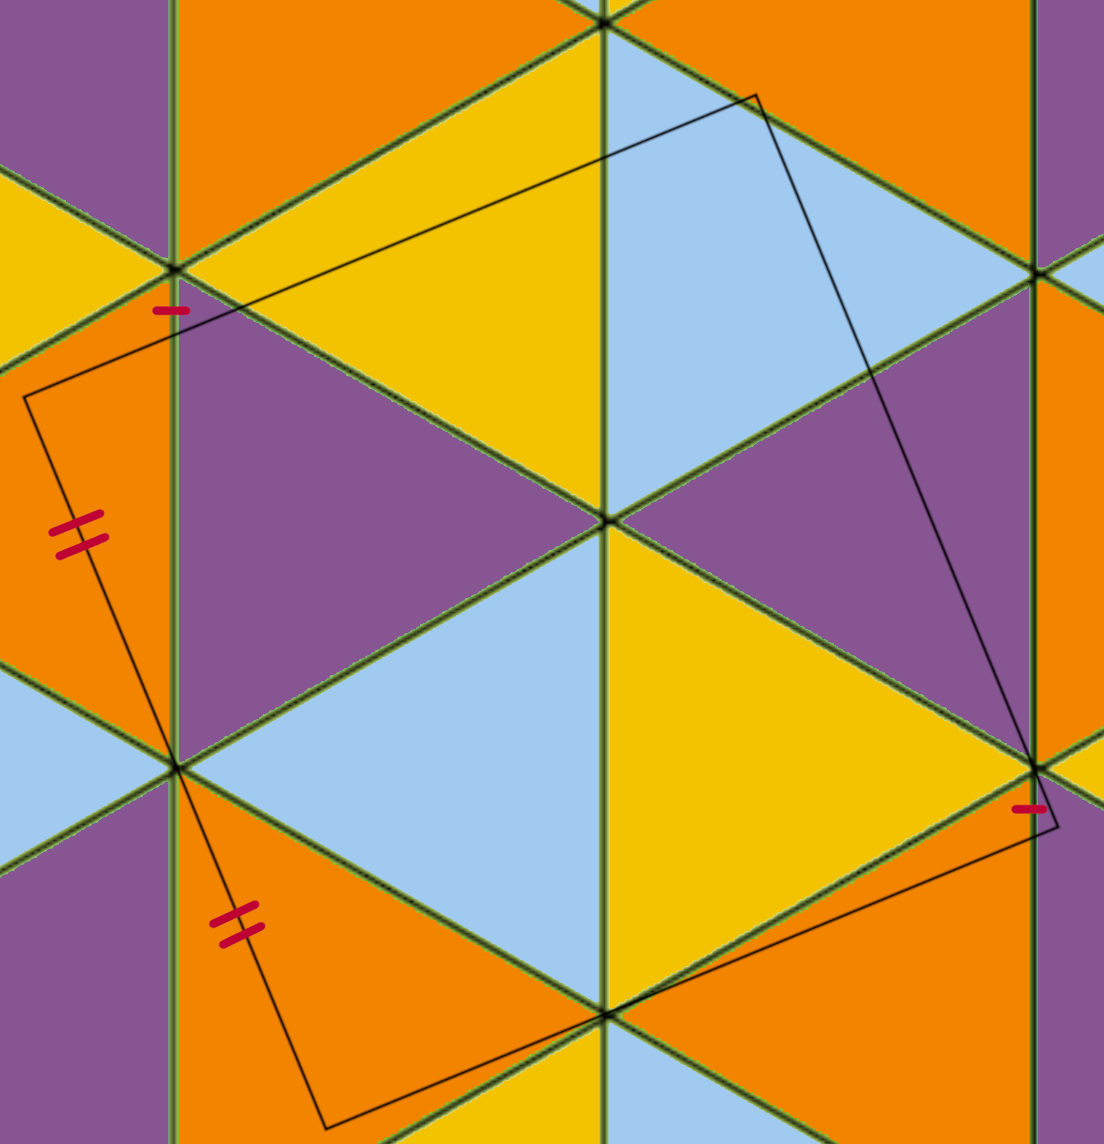
\includegraphics[scale=0.5]{triangle_land_squared}
\par\end{center}

The area inside this square covers every part of every color of triangle.
(The coverings of the purple and orange faces are each split among
three different copies of the triangle.) Therefore, by restricting
the full tiling fold to just this square, we obtain a complete wrapping
of this square around a tetrahedron. It can be checked manually that
this restriction does \emph{not }require the paper to intersect itself.

A brute-force computer search suggests that this is the smallest square
with this property. Its side length (we state without proof) is

\[
3\sqrt{\frac{7+2\sqrt{3}}{37}}\approx1.5954065\dots
\]

I conjecture that this is the most efficient way to fold a tetrahedron
from a square.

\section{Other polyhedra}

Unfortunately, the entire plane does not perfectly wrap around other
polyhedra. Instead we introduce the notion of a \emph{redundant net:}
\begin{defn}
A \emph{redundant net} of a polyhedron $P$ is a partial tiling of
the plane by labeled faces of $P$, such that a fold can map the labeled
faces onto the corresponding faces of $P$, possibly with the paper
intersecting itself.
\end{defn}

A polyhedron can have many redundant nets. This suggests a brute force
method:

\noindent\fbox{\begin{minipage}[t]{1\columnwidth - 2\fboxsep - 2\fboxrule}%
\textbf{Algorithm: searching for efficient foldings of a polyhedron
$P$}

Repeat:

$\hspace{1em}$1. Generate a random redundant net of $P$. (Be careful
-- since folding always increases distances, some otherwise valid
nets are impossible to actually fold. Our code checks that every pair
of vertices is at least as far apart on the square as on the surface
of the polyhedron. The diagrams below were then manually checked to
be foldable, in case this isn't sufficient.)

$\hspace{1em}$2. Via random search followed by gradient descent,
find a small square that covers every part of every face of $P$ in
the redundant net.%
\end{minipage}}

The random search in step 2 is fairly naive. In our implementation,
first several dozen squares are randomly placed on the redundant net.
Via binary search, we find for each square the smallest scaling of
it that covers the polyhedron. Finally, we use the third-party module
scipy to perform a final gradient descent. It is plausible that this
search could be vastly sped up by a superior algorithm.

Here are the results of running this algorithm for several hours on
the octahedron, dodecahedron, and icosahedron. Unlike for the tetrahedron,
I do not conjecture that any of these are optimal. The dodecahedron
fold in particular might even be locally improvable by ``hinging''
the bottommost yellow pentagon.
\begin{center}
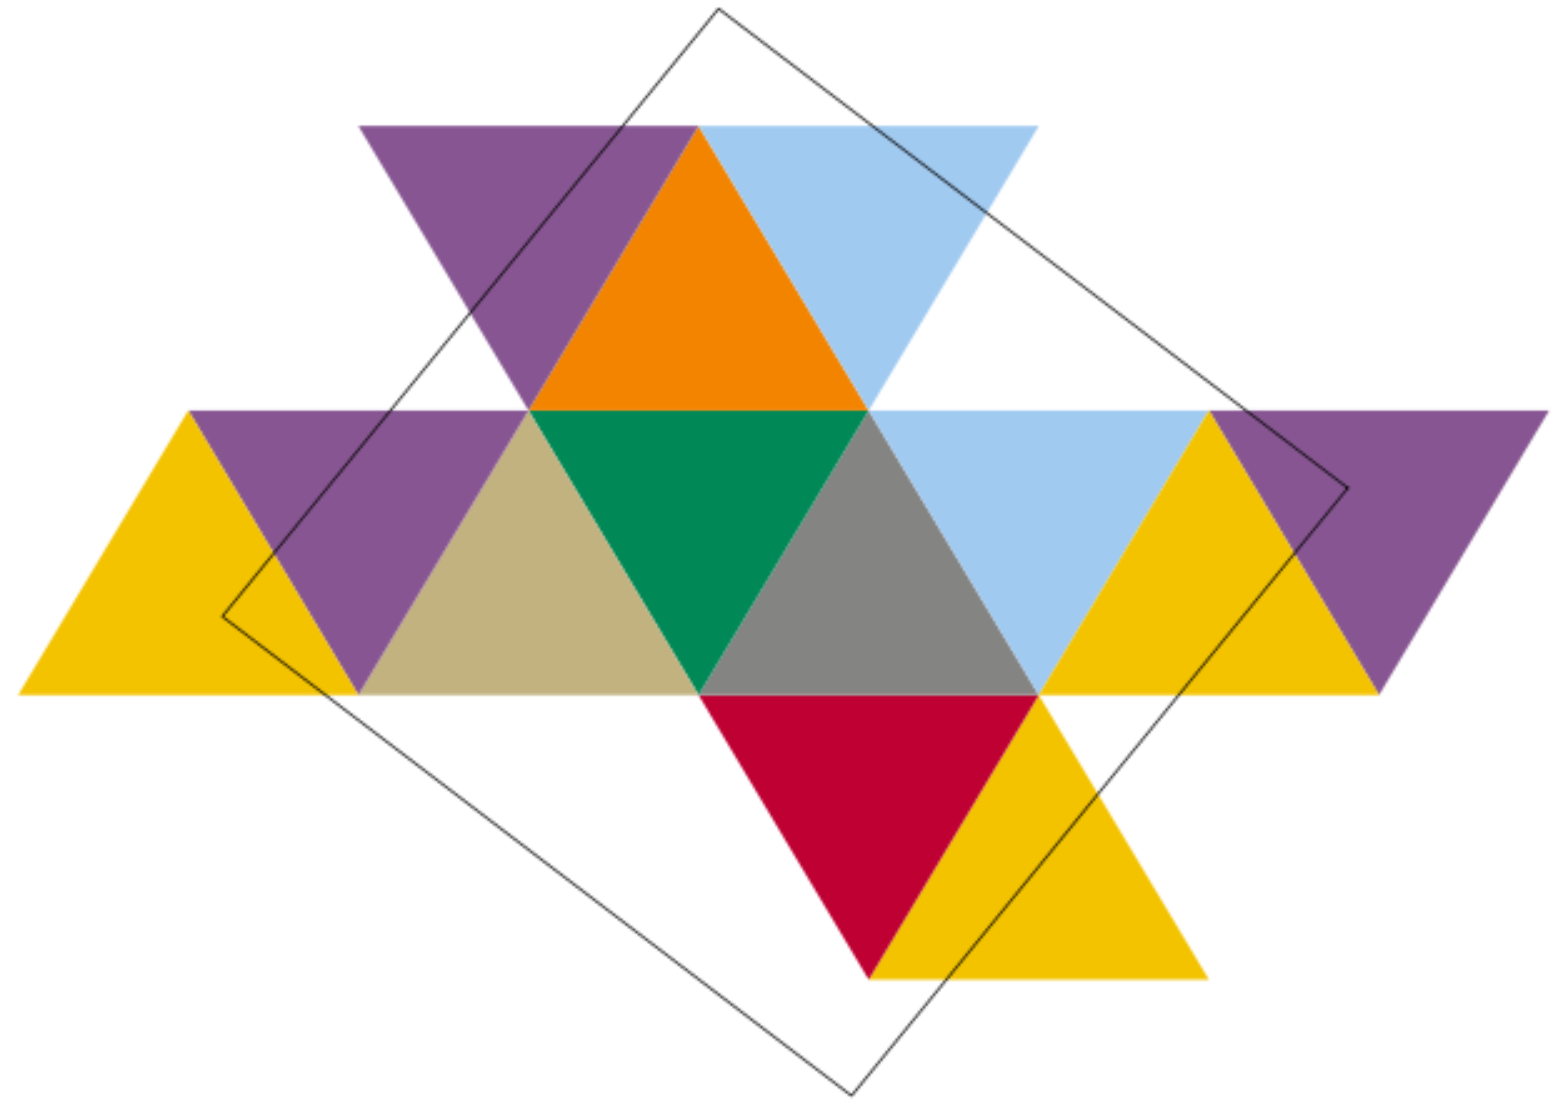
\includegraphics[scale=0.5]{octarecord}
\par\end{center}

\begin{center}
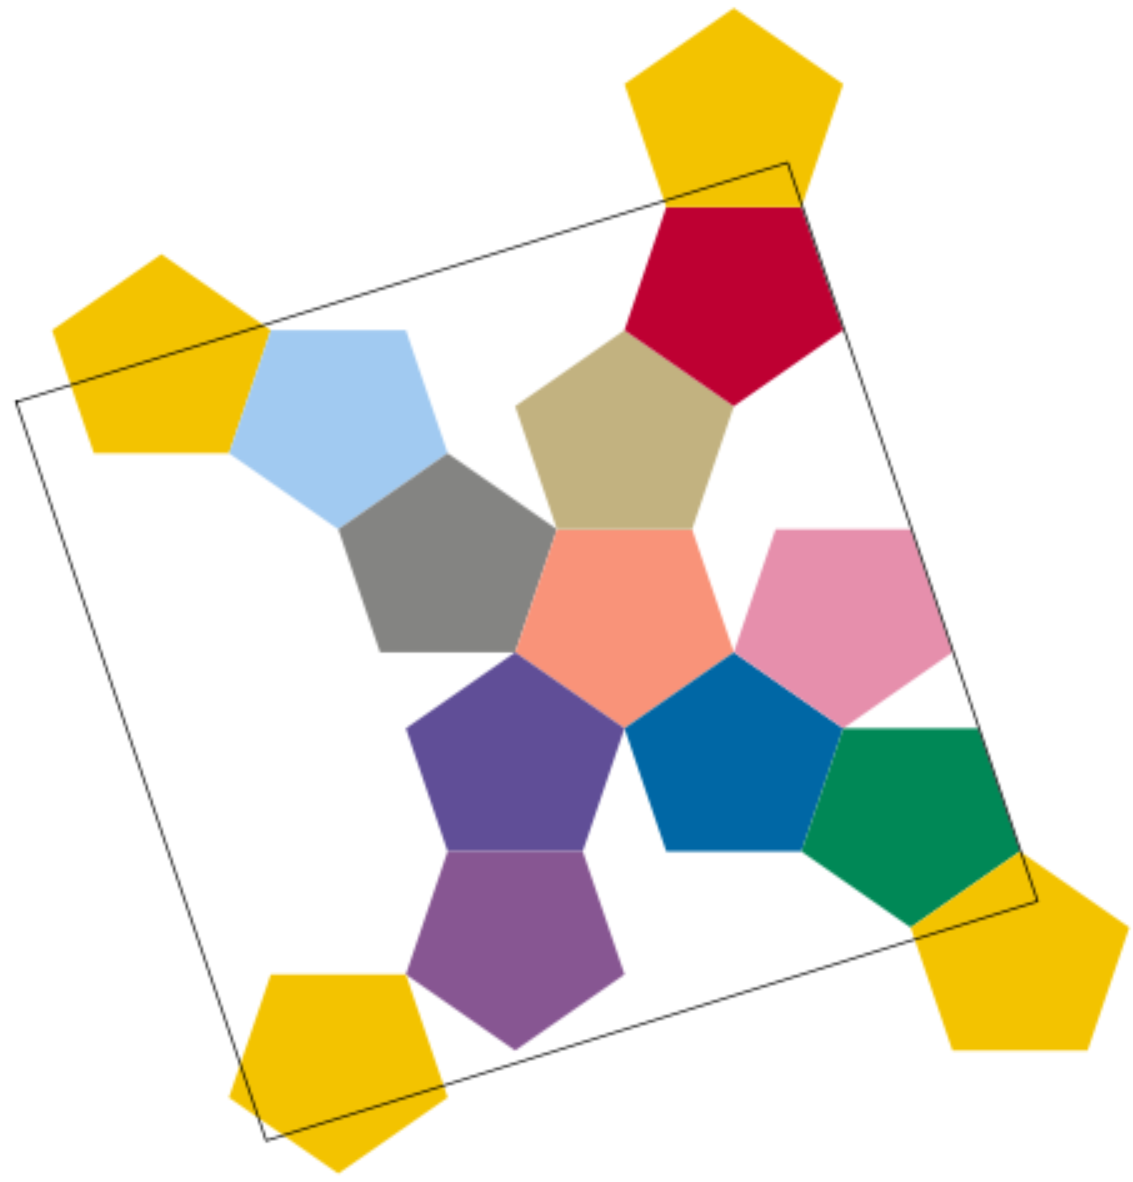
\includegraphics[scale=0.5]{dodecarecord}
\par\end{center}

\begin{center}
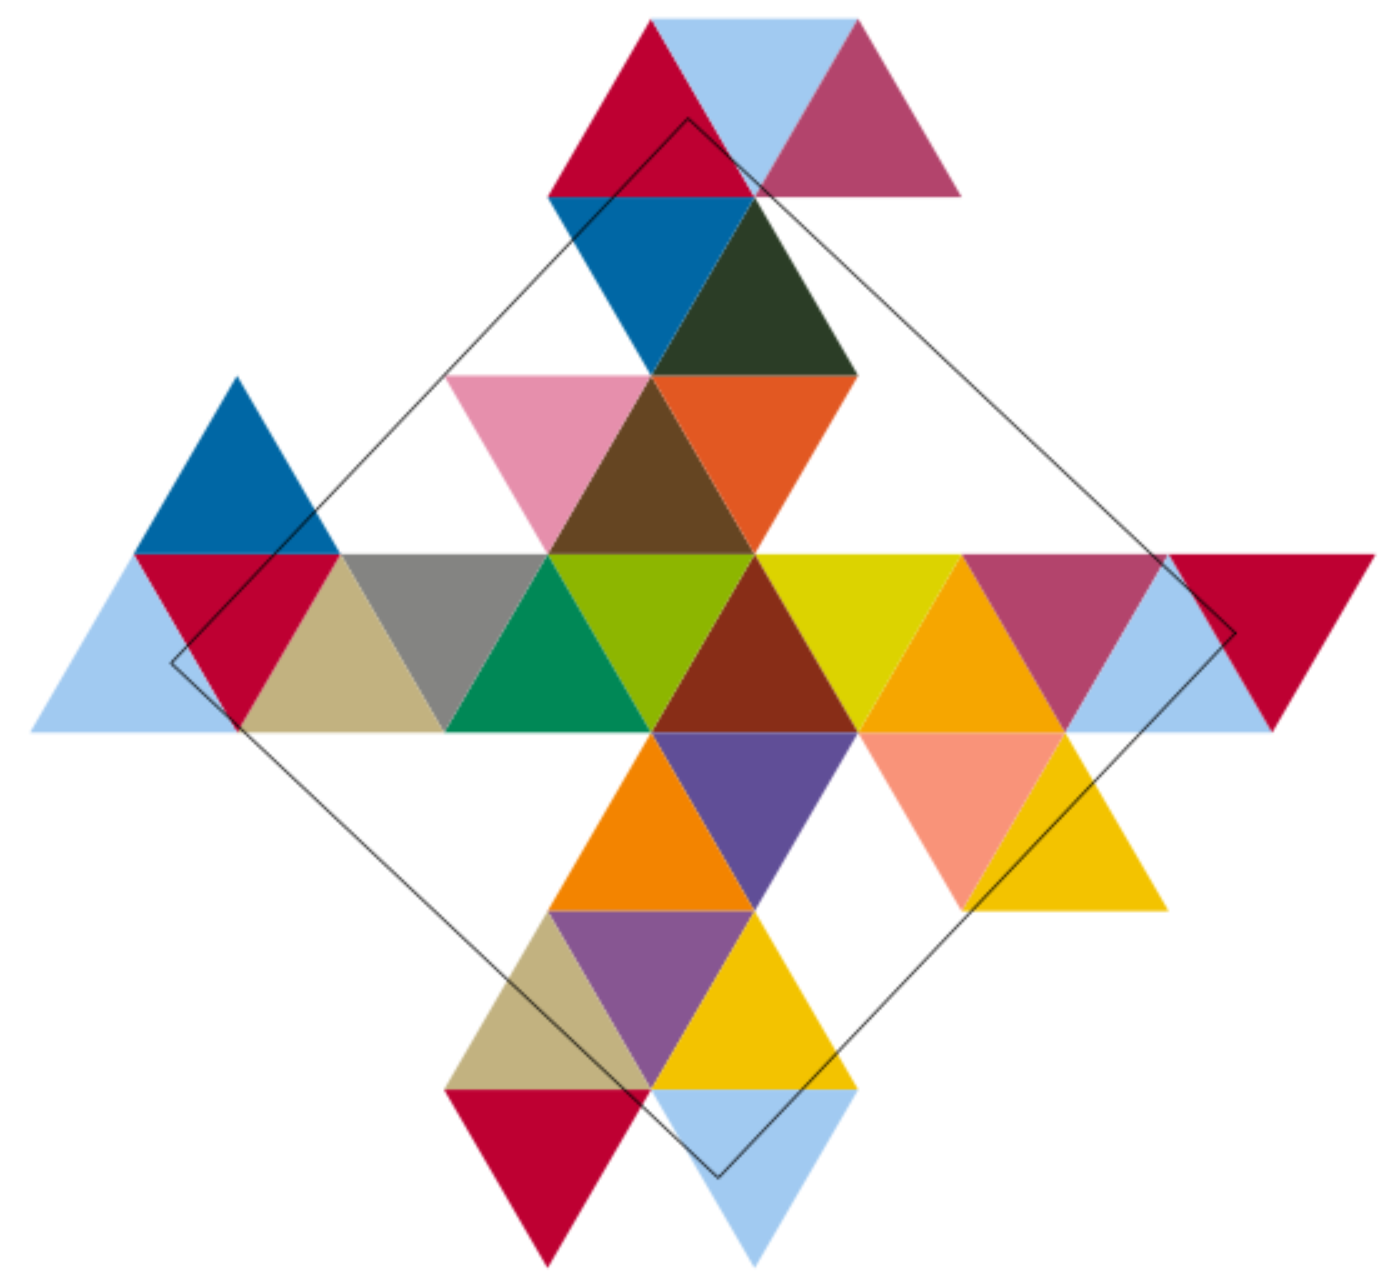
\includegraphics[scale=0.5]{icosarecord}
\par\end{center}

The side lengths of these squares are at most 2.35557, 6.00181, and
3.63663, respectively.

Python code at\url{https://github.com/6849-2020/efficient-polyhedra-folds/blob/main/foldingPolyhedra.py}allows
you to run this algorithm on any polyhedron of your choice, as well
try paper shapes other than square.

\section{A conditional lower bound for the tetrahedron}

One classical lower bound on folding a tetrahedron is known:
\begin{thm}
One cannot fold a unit tetrahedron from a square of side length less
than $\sqrt{2}$.
\end{thm}

\begin{proof}
No matter which point $x$ on the tetrahedron the center of the square
maps to, there is some point distance $\geq1$ away on the surface
of the tetrahedron. Therefore, to cover this point, the square must
have a point distance $\geq1$ from its center. It follows that the
side length of the square is $\geq\sqrt{2}$.
\end{proof}
We have not improved this bound unconditionally. However, we can show
a conditional bound for folding patterns containing what we call a
``diamond'' configuration. For the purpose of exposition, let us
do an example:
\begin{fact}
The partial folding shown below, with two adjacent tetrahedron faces
already mapped, cannot be extended to cover the whole tetrahedron.

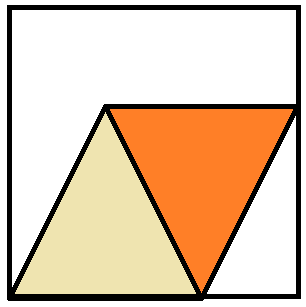
\includegraphics{diamond_pattern}
\end{fact}

\begin{proof}
(Informal) We have already chosen points on the square $p_{A},p_{B},p_{C},p_{D}$
mapping to the four vertices $A,B,C,D$ of the tetrahedron. Folding
cannot increase distances. So for any point $T$ on the tetrahedron,
it must be covered by a point $p_{T}$ on the square satisfying $d(p_{T},p_{A})\geq d_{\text{tetrahedron}}(T,A)$
and analogously for $B,C,D$.

But (I claim here without proof) there exists a point $x$ on the
tetrahedron such that these bounds rule out the entire square. So
this point $x$ cannot be covered.
\end{proof}
We shall use this technique to prove the following restricted lower
bound:
\begin{thm}
Suppose a folding of a tetrahedron from a square contains a ``diamond''
configuration as shown above. Then the side length of the square is
more than 1.55.
\end{thm}

Using a proof of the form above, we can rule out a single possible
placement of a diamond in the side-1.55 square. In fact, we can do
a little more. If the proof has any slack in the inequalities, then
we can rule out a small neighborhood of possible diamond locations.
The following lemma makes this explicit.
\begin{lem}
Parameterize the space of possible diamond positions by $x,y,\theta$,
where $(x,y)$ is the center of the diamond and $\theta$ is its angle.
Say a diamond with center $(x,y)$ and angle $\theta$, having vertices
$p_{A},p_{B},p_{C},p_{D}$, is placed overlapping a square $S$.

$(a)$ Suppose for some constant $\delta$ that some vertex of the
diamond -- one of $p_{A},p_{B},p_{C},p_{D}$ -- lies outside the
square $S$ by distance more than $(\sqrt{2}+\frac{\sqrt{3}}{2})\delta$.
Then that vertex still lies outside the square even if the parameters
$x,y,\theta$ are first each adjusted by as much as $\delta$.

$(b)$ Suppose for some constant $\delta$ there exists a tetrahedron
point $T$ such that \emph{no }point $p_{T}\in S$ satisfies all four
of these bounds: $d(p_{T},p_{A})>d_{\text{tetrahedron}}(T,A)+(\sqrt{2}+\frac{\sqrt{3}}{2})\delta$
and analogously for $B,C,D$. Then the diamond folding cannot be extended
to cover point $T$, even if the parameters $x,y,\theta$ of the diamond
are first each adjusted by as much as $\delta$.
\end{lem}

\begin{proof}
If the $x,y,\theta$ parameters of the diamond change by at most $\delta$
each, then every vertex of the diamond $p_{A},p_{B},p_{C},p_{D}$
moves by at most $\sqrt{2}\delta$ (from changing $x$ and $y$),
plus $\frac{\sqrt{3}}{2}\delta$ (from the rotation by $\theta$ applied
to the vertices $\frac{\sqrt{3}}{2}$ from the center of the diamond).
This proves (a). This also shows that moving the diamond weakens the
inequalities $d(p_{T},p_{A})>d_{\text{tetrahedron}}(T,A)+(\sqrt{2}+\frac{\sqrt{3}}{2})\delta$
in (b) to merely $d(p_{T},p_{A})>d_{\text{tetrahedron}}(T,A)$, which
is still enough to apply the proof of the previous fact. This proves
(b).
\end{proof}
To prove our main lower bound, we use the lemma to incrementally rule
out all possible locations of the diamond. The configuration space
for the $x,y,\theta$ parameters of the diamond is a box $[0,1.55]\times[0,1.55]\times[0,\tau/2]$.
Now run the following algorithm:

$ $

\noindent\fbox{\begin{minipage}[t]{1\columnwidth - 2\fboxsep - 2\fboxrule}%
\textbf{Algorithm: ruling out a box $[x_{min},x_{max}]\times[y_{min},y_{max}]\times[\theta_{min},\theta_{max}]$}

1. Let $x,y,\theta$ be the center of this box.

2. Via randomly probing tetrahedron points $T$, search for a proof
using the lemma showing that $T$ cannot be covered whenever the diamond
pattern lies in the box.

3. If no proof is found quickly, then cut the box along each axis
to obtain 8 smaller boxes, and recursively run this algorithm on each
smaller box.%
\end{minipage}}

$ $

If the algorithm halts on the original box $[0,1.55]\times[0,1.55]\times[0,\tau/2]$,
then the theorem is proved. In short: it does. We omit the execution
for brevity, as the program checks approximately ten thousand sub-boxes.
See the github for code. It is plausible that running the code for
longer could prove a stronger bound than 1.55. It would be interesting
to take this technique all the way to the conjectured upper bound
$1.5954065\dots$.

\section{Future Work}

A simple next step: run my code to search for the smallest rectangle
with a given side length ratio that covers a cube. Compare the results
to those in \cite{cole2013wrapping}.

Though the configuration-space-search proof in the previous section
is unwieldy and requires computer time, it may open the door to lower
bounds for other simple computational geometry problems.

Also, a natural question to ask: is the problem ``What is the smallest
square that folds to cover the polyhedron $P$'' \emph{computable}?
It does not obviously fall to Tarski's proof that the theory of the
reals is decidable.

\bibliographystyle{plain}
\bibliography{\string"bibliography\string"}


\section{Appendix: TODOs if this gets published}

As an addendum, there are some rough spots in this paper to fix if
we want to publish this result.
\begin{enumerate}
\item Finally now that I've updated my code to handle paper shapes other
than a square, try to improve the wrapping-a-rectangle-around-a-cube
bounds from \cite{cole2013wrapping}. Or try to wrap a triangle around
a cube, etc.
\item Give a quick proof in an appendix that the tetrahedron folding achieves
side length $3\sqrt{\frac{7+2\sqrt{3}}{37}}$.
\item Is there a procedural way to check that the final results for the
octahedron/dodecahedron/icosahedron can be folded without stretching
or overlapping paper? I manually checked them here, but I'm not sure
how to turn that into a proof.
\item Convert the conditional 1.55 lower bound proof to some text file format
so that it can be quickly computer checked for correctness. Also write
the ``check for correctness'' code in a good style so that it's clear
that if it outputs True, then the proof is correct.
\item Make the Platonic solid folds colorblind accessible, e.g. label each
face with a number.
\end{enumerate}

\end{document}
